All code for this section can be found within the appendices.

\subsection{Part a}

The frequency response of the filter is given by the following:

\begin{gather*}
	y[n]=\frac{1}{11}\sum_{k=0}^{10} x[n-k] \\
	\text{Converting to the Frequency Domain} \\
	H(j\hat{\omega})=\frac{1}{11}\sum_{k=0}^{10} e^{-j\hat{\omega}k} \\
	\text{Sum of a Geometric Series} \\
	\sum_{k=0}^{L-1} a^k=\frac{1-\alpha^L}{1-\alpha} \\
	H(j\hat{\omega})=\frac{1}{L}(\frac{1-e^{-j\hat{\omega}L}}{1-e^{-\hat{\omega}}})\\
	\text{Taking out a factor of } e^{\frac{-j\hat{\omega}L}{2}} \text{ from the
	numerator} \\
	\text{and } e^{\frac{-j\hat{\omega}}{2}} \text{from the denominator:} \\
	H(j\hat{\omega})=\frac{1}{L}(\frac{e^{\frac{-j\hat{\omega}L}{2}}(e^{\frac{j\hat{\omega}}{2}}-e^{\frac{-j\hat{\omega}L}{2}})}{e^{\frac{-j\hat{\omega}}{2}}(e^{\frac{j\hat{omega}}{2}}-e^{-\frac{j\hat{\omega}}{2}})}) \\
	H(j\hat{\omega})=(\frac{\sin(\frac{\hat{\omega
	L}}{2})}{L\sin(\frac{\hat{\omega}}{2})})e^{\frac{-j\hat{\omega}(L-1)}{2}}
\end{gather*}

As in the code shown, the Dirichlet function is used for the computation of the
magnitude. The output plot can be seen in the first plot in Figure
\ref{fig:Q2Img}, found below.

\begin{figure}[H]
	\centering
	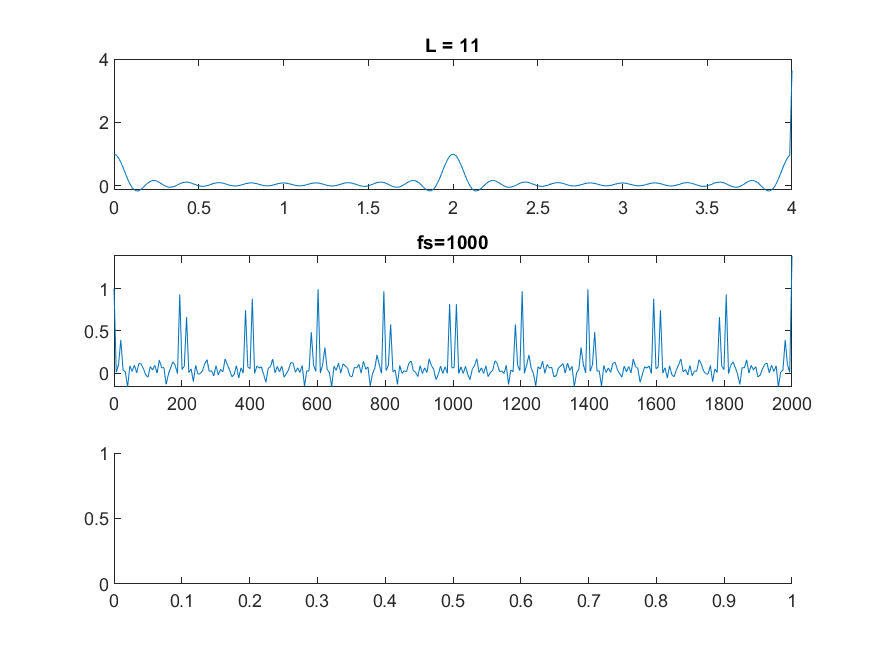
\includegraphics[width=0.8\textwidth]{images/Q2.png}
	\caption{The output from Q2 Part 1, Part 2, and Part 3}
	\label{fig:Q2Img}
\end{figure}
